\chapter[Forme paramétrique à forme simplifiée]{Passage de la forme simplifiée à la forme paramétrique d'une ellipse}
\begin{figure}[h!]
\centering
\resizebox{0.8\textwidth}{!}{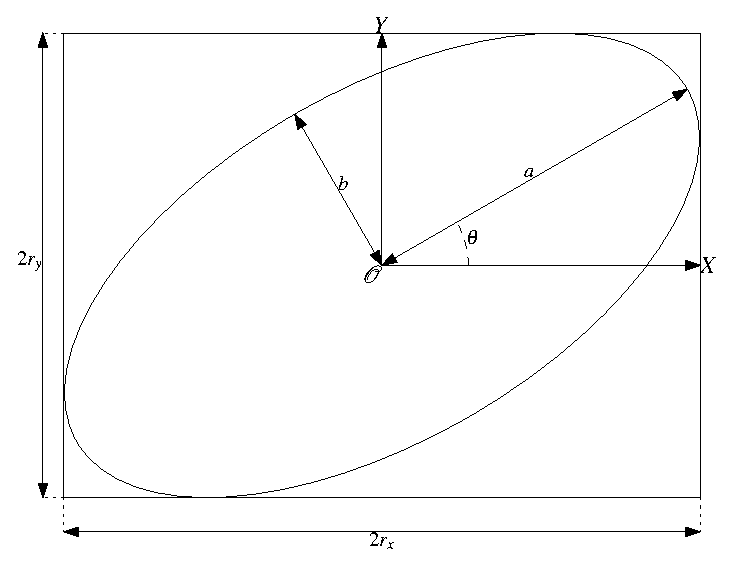
\includegraphics{img/ellipse_annexe.eps}}
\caption[Trajectoire elliptique]{\label{chap1:fig:ell_c}Trajectoire elliptique générale $\mathbf{p}_e$ dans un plan $XY$,centrée à l'origine, orientée d'un angle $\theta$ et ayant respectivement des longueur de grand et petit rayons $a$ et $b$.}
\end{figure}
Une ellipse centrée à l'origine dans un plan $XY$, ayant une longueur de grand rayon de $a$ et une longueur de petit rayon de $b$ et orientée avec un angle de $\theta$ par rapport à l’abscisse $X$  est représenté à la figure \ref{chap1:fig:ell_c} et son équation paramétrique temporelle s'écrit 
\begin{align}
\mathbf{p}_e(t) =
\begin{bmatrix}
a\cos(\theta)\cos(\omega t+\phi)-b\sin(\theta)\sin(\omega t+\phi)\\
a\sin(\theta)\cos(\omega t+\phi)+b\cos(\theta)\sin(\omega t+\phi)
\end{bmatrix}, \label{annC:eq:ell_base}
\end{align}

où $t$ est le temps en seconde et $\omega$ est ici appelée la fréquence d'oscillation angulaire et décrit combien de fois par seconde (s) un tour complet (oscillation) autour de l’ellipse est effectué par un point suivant la trajectoire $\mathbf{p}_e(t)$ en rad/s. Conséquemment, la période de cette trajectoire est de $T = \frac{2\pi}{\omega}$ s. Les valeurs $\phi$ est en rad et  permet d'établir la position initiale de la trajectoire sur l'ellipse. 

La formulation de $\mathbf{p}_d(t)$ en (\ref{annC:eq:ell_base}) est très longue et peut être simplifiée sous la forme \begin{align}
\mathbf{p}_d(t) = \begin{bmatrix}
r_x\sin(\omega t+\phi_x)\\
r_y\sin(\omega t+\phi_y)
\end{bmatrix}.
\label{annC:eq:gen_ell_simp}
\end{align}
\begin{multline}
a\cos(\theta)\left(\cos(\tau)\cos(\phi)-\sin(\tau)\sin(\phi)\right)-b\sin(\theta)\left(\sin(\tau)\cos(\phi)+\cos(\tau)\sin(\phi)\right) \\ = r_x(\sin(\tau)\cos(\phi_x)+\cos(\tau)\sin(\phi_x))
\end{multline}
\begin{multline}
a\sin(\theta)\left(\cos(\tau)\cos(\phi_a)-\sin(\tau)\sin(\phi_a)\right)+b\cos(\theta)\left(\sin(\tau)\cos(\phi_b)+\cos(\tau)\sin(\phi_b)\right)  \\ = r_y(\sin(\tau)\cos(\phi_y)+\cos(\tau)\sin(\phi_y)),
\end{multline}
\begin{align}
a\cos(\theta)\cos(\phi)-b\sin(\theta)\sin(\phi)=r_x\sin(\phi_x)\\
-a\cos(\theta)\sin(\phi)-b\sin(\theta)\cos(\phi)=r_x\cos(\phi_x)\\
\bar{\mathcal{V}}
\end{align}
où $\tau=\omega t$ est utilisé afin de raccourcir la longueur des termes.



















